\documentclass[10pt]{book}
\usepackage[sectionbib]{natbib}
\usepackage{array,epsfig,fancyhdr,rotating}
\usepackage[driverfallback=dvipdfm]{hyperref}
\usepackage{soul} %for strikeout
\usepackage{csquotes}
%%%%%%%%%%%%%%%%%%%%%%%%%%%%%%%%%%%%%%%%%%%%%%%%%%%%%%%%%%%%%%%%%%%%%%%%%%%%%%%%%%%%%%%%%%%%%%%%%%%%%%%%%%%%%%%%%%%%%%%%%%%%

\textwidth=31.9pc
\textheight=46.5pc
\oddsidemargin=1pc
\evensidemargin=1pc
\headsep=15pt
%\headheight=.2cm
\topmargin=.6cm
\parindent=1.7pc
\parskip=0pt

\usepackage{amsmath}
\usepackage{amssymb}
\usepackage{amsfonts}
\usepackage{multirow}
\usepackage{amsthm}
\usepackage[export]{adjustbox}

\setcounter{page}{1}
\newtheorem{theorem}{Theorem}
\newtheorem{lemma}{Lemma}
\newtheorem{corollary}{Corollary}
\newtheorem{proposition}{Proposition}
\theoremstyle{definition}
\newtheorem{definition}{Definition}
%\newtheorem{proof}{Proof}
\newtheorem{example}{Example}
\newtheorem{remark}{Remark}
\pagestyle{fancy}

% List labels
\usepackage{scrextend}
\addtokomafont{labelinglabel}{\sffamily}

% Reference labels in the online appendix
\usepackage{xr}
\externaldocument{mdi-ss-supp}

%%%%%%%%%%%%%%%%%%%%%%%%%%%%%%%%%%%%%%%%%%%%%%%%%%%%%%%%%%%%%%%%%%%%%%%%%%%%%%%%%%%%%%%%%%%%%%%%%%%%%%%%%%%%%%%%%%%%%%%%%%%%
\pagestyle{fancy}
\def\n{\noindent}
\lhead[\fancyplain{} \leftmark]{}
\chead[]{}
\rhead[]{\fancyplain{}\rightmark}
\cfoot{}
\renewcommand{\headrulewidth}{0pt}

%%%%%%%%%%%%%%%%%%%%%%%%%%%%%%%%%%%%%%%%%%%%%%%%%%%%%%%%%%%%%%%%%%%%%%%%%%%%%%%%%%%%%%%%%%%%%%%%%%%%%%%%%%%%%%%%%%%%%%%%%%%%
%%%%%%%%%%%%%%%%%%%%%%%%%%%%%%%%%%%%%%%%%%%%%%%%%%%%%%%%%%%%%%%%%%%%%%%%%%%%%%%%%%%%%%%%%%%%%%%%%%%%%%%%%%%%%%%%%%%%%%%%%%%%

\begin{document}

%%%%%%%%%%%%%%%%%%%%%%%%%%%%%%%%%%%%%%%%%%%%%%%%%%%%%%%%%%%%%%%%%%%%%%%%%%%%%%%%%%%%%%%%%%%%%%%%%%%%%%%%%%%%%%%%%%%%%%%%%%%%
%%%%%%%%%%%%%%%%%%%%%%%%%%%%%%%%%%%%%%%%%%%%%%%%%%%%%%%%%%%%%%%%%%%%%%%%%%%%%%%%%%%%%%%%%%%%%%%%%%%%%%%%%%%%%%%%%%%%%%%%%%%%

\renewcommand{\baselinestretch}{2}

\markright{ \hbox{\footnotesize\rm Statistica Sinica
%{\footnotesize\bf 24} (201?), 000-000
}\hfill\\[-13pt]
\hbox{\footnotesize\rm
%\href{http://dx.doi.org/10.5705/ss.20??.???}{doi:http://dx.doi.org/10.5705/ss.20??.???}
}\hfill }

\markboth{\hfill{\footnotesize\rm JASON POULOS AND RAFAEL VALLE} \hfill}
{\hfill {\footnotesize\rm MISSING DATA IMPUTATION} \hfill}

\renewcommand{\thefootnote}{}
$\ $\par

%%%%%%%%%%%%%%%%%%%%%%%%%%%%%%%%%%%%%%%%%%%%%%%%%%%%%%%%%%%%%%%%%%%%%%%%%%%%%%%%%%%%%%%%%%%%%%%%%%%%%%%%%%%%%%%%%%%%%%%%%%%%

\fontsize{12}{14pt plus.8pt minus .6pt}\selectfont \vspace{0.8pc}
\centerline{\large\bf MISSING DATA IMPUTATION FOR SUPERVISED LEARNING}
%\vspace{2pt} \centerline{\large\bf }
\vspace{.4cm} \centerline{Jason Poulos and Rafael Valle} \vspace{.4cm} \centerline{\it
University of California, Berkeley} \vspace{.55cm} \fontsize{9}{11.5pt plus.8pt minus
.6pt}\selectfont

%%%%%%%%%%%%%%%%%%%%%%%%%%%%%%%%%%%%%%%%%%%%%%%%%%%%%%%%%%%%%%%%%%%%%%%%%%%%%%%%%%%%%%%%%%%%%%%%%%%%%%%%%%%%%%%%%%%%%%%%%%%%

\begin{quotation}
\noindent {\it Abstract:}
This paper compares methods for imputing missing categorical data for classification tasks using random forests, decision trees, and artificial neural networks (ANNs). Researchers analyzing survey data typically choose decision trees or random forests for classification tasks, largely because these models do not require imputing missing data nor encoding categorical variables, unlike ANNs or other classifiers. We experiment on two benchmark datasets with missing categorical data, comparing the three classifiers trained on non-imputed (i.e., one-hot encoded) or differently imputed data with different degrees of missing not at random (MNAR) perturbation. The results of the experiments show that for non-imputed models, perturbation produces a considerable decrease in prediction accuracy relative to models trained on imputed data due to correlation between features. Additionally, we find that for imputed models, MNAR perturbation can improve prediction accuracy by regularizing the training data. \par

\vspace{9pt}
\noindent {\it Key words and phrases:} % alphabetical order
artificial neural networks (ANNs), decision trees,  imputation methods, missing data, missing not at random (MNAR), prediction intervals, random forests, survey data
\par
\end{quotation}\par



\def\thefigure{\arabic{figure}}
\def\thetable{\arabic{table}}

\fontsize{12}{14pt plus.8pt minus .6pt}\selectfont

\newpage %move intro to second page

\setcounter{chapter}{1}
\setcounter{equation}{0} %-1
\noindent {\bf 1. Introduction} 

Missing data is a common problem in survey data in various domains, such as social science and marketing. Sources of missing data in surveys include nonresponse and attrition in longitudinal surveys. For supervised classification tasks, the objective is to fit a model on categorically labeled training data in order to categorize new examples. The ability of researchers to accurately fit a model model may be compromised by missing data, depending on the underlying missing data mechanism. In this paper, we focus on data that are missing not at random (MNAR), which occurs when the probability of an example having a missing value depends on the missing data itself. There is an inherent nonidentifiability problem when the missing data mechanism is MNAR because we cannot observe the true value of missing data \citep[Chap.~6]{tsiatis2007}. Nonresponse in surveys is typically handled by imputation methods, which are used to estimate a value for missing data. However, imputation methods assume data missing at random (MAR), which occurs when the probability of missingness depends only on the observed data. 

The objective of the present study is to compare the out-of-sample performance of three popular machine learning classifiers --- decision trees, random forests, and artificial neural networks (ANNs) --- trained on differently-imputed or non-imputed (i.e., one-hot encoded) survey datasets that contain various degrees of MNAR missing data. Decision trees and random forests are typically used for survey data because missing data must be preprocessed to be suited for models that require numerical input, such as ANNs. Imputation methods that assume data at MAR when the data is in fact MNAR can bias model estimates. The results of the study will provide guidance to applied researchers on how to handle missing data in survey datasets and which classifier to use. 

This manuscript is organized as follows: Section 2 describes missing data mechanisms and imputation methods; Section 3 describes our experiments on two benchmark datasets and discusses the results; Section 4 concludes and offers areas for future research. 

\par

\lhead[\footnotesize\thepage\fancyplain{}\leftmark]{}\rhead[]{\fancyplain{}\rightmark\footnotesize\thepage}%Put this line in Page 2

\setcounter{chapter}{2}
\setcounter{equation}{0} %-1
\noindent {\bf 2. Missing data and imputation methods}

In this section, we describe the missing data mechanisms underlying patterns of missing data common to survey datasets. We then review popular methods of handling missing data.

\par
\noindent {\bf 2.1. Missing data patterns and mechanisms}

It is important to first distinguish between missing data patterns, which describe which values are observed and which are missing, and missing data mechanisms, which describe the the probability of missingness  \citep[Chap.~1]{little2014}. Common missing data patterns in surveys typically include unit nonresponse, where a subset of participants do not complete the survey, and item nonresponse, where missing values are concentrated on particular questions. In opinion polls, nonresponse may reflect either refusal to reveal a preference or lack of a preference \citep{de2003prevention}. 

Imputing missing values in situations where missing data hide values that are useful for classification tasks can help improve prediction accuracy. Understanding the missing data mechanisms underlying patterns of missing data is crucial since properties of imputation methods depend on the nature of these mechanisms. Following the notation of \cite[Chap.~1]{little2014}, let $Y = y_{ij}$ be a $(n \times K)$ dataset with each row $y_i = (y_{i1}, \ldots, y_{iK})$ the set of $y_{ij}$ values of feature $Y_j$ for example $i$. Let $Y_{\mathrm{obs}}$ define observed values of $Y$ and $Y_{\mathrm{mis}}$ define missing values. Define the missing data identity matrix $M = m_{ij}$, where $m_{ij} = 1$ if $y_{ij}$ is missing and $m_{ij} = 0$ if $y_{ij}$ is nonmissing. The missing data mechanism is missing completely at random (MCAR) if the probability of missingness is independent of the data, or $f(M | Y, \phi) = f(M | \phi)$ for all $Y, \phi$, where $\phi$ denotes unknown parameters. The MAR assumption is less restrictive than MCAR in that that the probability of missingness depends only on the observed data, $f(M | Y, \phi) = f(M | Y_{\mathrm{obs}}, \phi)$ for all $Y_{\mathrm{mis}}, \phi$. We are primarily interested in the MNAR assumption that the probability of missingness may also depend on the unobserved data, $f(M | Y, \phi) = f(M | Y_{\mathrm{mis}}, \phi)$ for all $Y_{\mathrm{mis}}, \phi$. Researchers typically assume data is MAR, which mitigates the identifiability problems of MNAR because the probability of missingness depends on data that are observed on all individuals \citep[Chap.~6]{tsiatis2007}. 

\par			
\noindent {\bf 2.2. Imputation methods} \label{section:techniques} 

Complete-case analysis (i.e., simply discarding examples with missing values) wastes information and biases estimates unless the data are MCAR. Since there is no way to distinguish whether the missing data are MCAR or MNAR from the observed data, a natural strategy is to impute missing values and then proceed as if the imputed values are true values. Imputation methods that rely on explicit model assumptions include \emph{mean or mode replacement}, which substitutes missing values with the mean (for quantitative features) or mode (for qualitative features) of the feature vector, and \emph{prediction model} imputation, which replaces missing values with the predicted values from a regression of $Y_{\mathrm{mis}}$ on $Y_{\mathrm{obs}}$. Explicit modeling methods assume the data are MAR while implicit modeling methods, which are algorithmic in nature and rely only on implicit assumptions, generally do not assume the underlying missing data mechanism. Implicit methods include \emph{random replacement}, where an example with missing data is randomly replaced with another complete example randomly sampled, and \emph{hot deck} imputation, where missing values are replaced by ``similar'' nonmissing values. Hot deck imputation can be implemented by computing the $k$-nearest-neighbors ($k$-NN) of an example with missing data and assigning the mode of the $k$-neighbors to the missing data. \cite{batista2003analysis} use this procedure and find $k$-NN imputation can outperform internal methods used by decision trees to treat missing data and summary statistic imputation. \cite{li2004} propose a hot deck imputation method based on fuzzy $k$-means. 

\cite{silva2011} empirically compare imputation using ANNs with mean/mode imputation, regression models (logistic regression and multiple linear regression), or hot deck, and find the ANNs model performs the best on datasets with categorical variables. 

\par
\noindent {\bf 2.3. One-hot encoding for missing data} 

A natural strategy in dealing with missing data for supervised learning problems is one-hot encoding. Instead of imputing missing data, one-hot encoding creates a binary feature vector that indicates missing values. For categorical features, one-hot encoding simply treats a missing value symbol (e.g, ``?") as a category when the categorical features are binarized. For continuous features, missing values are set to a constant value and a missingness indicator is added to the feature space. One-hot encoding for missing data yields biased estimates when the features are correlated, which is often the case with survey data, even when data are MCAR \citep{jones1996}. 

\par

%%%%%%%%%%%%%%%%%%%%%%%%%%%%%%%%%%%%%%%%%%%%%%%%%%%%%%%%%%%%%%%%%%%%%%%%%%%%%%%%%%%%%%%%%%%%%%%%%%%%%%%%%%%%%%%%%%%%%%%%%%%%
%\newpage

\setcounter{chapter}{3}
\setcounter{equation}{0} %-1
\noindent {\bf 3. Experiments} 

In this section, we describe our experiment on two benchmark datasets with missing categorical data, comparing three popular classifiers --- ANNs, decision trees, and random forests--- trained on either non-imputed or differently imputed data with different degrees of MNAR perturbation.

\par
\noindent {\bf 3.1. Benchmark datasets}

We experiment on two benchmark datasets from the UCI Machine Learning Repository: the Adult dataset and Congressional Voting Records (CVRs) dataset \citep{Lichman2013}. The Adult dataset contains $N=48,842$ examples and 14 features (6 continuous and 8 categorical). Missing values in this dataset are survey nonresponses. The prediction task is to determine whether a person makes over \$50,000 a year. The CVRs dataset contains $N=435$ examples, each the voting record of a member of the $98^{th}$ U.S. House of Representatives for 16 key roll call votes. The dataset contains 16 categorical features with three possible values: ``yea'', ``nay'', and missing. Missing values in this dataset are not simply unknown, but represent values other up-or-down votes, such as voted present, voted present to avoid conflict of interest, and did not vote or otherwise make a position known. The prediction task is to classify party affiliation (Republican or Democrat). 

We randomly split each dataset $2/3$ for training and $1/3$ for testing. The state--of--the--art for the Adult dataset is a Naive Bayes classifier that achieves a 14.05\% generalization error after removing examples with missing values \citep{kohavi1996}. The CVRs dataset donor claims to achieve a 90-95\% accuracy using an incremental decision tree algorithm called STAGGER, although it is unknown to the authors what train-test split is used or how missing values are handled \citep{schlimmer1987,schlimmer1986}.

\par
\noindent {\bf 3.2. Patterns of missing data}

Uncovering missing data patterns in the datasets is will help to identify possible missing data mechanisms and select appropriate imputation methods. In the supplementary material (SM), Figure SM-\ref{fig:proportion-missing-adult} analyzes patterns of missing data in the Adult dataset, in which 7\% of the examples contain missing values. Missing data in the Adult dataset is due to item nonresponse, as missing values are concentrated in three of the categorical features --- \emph{Work class}, \emph{Occupation}, and \emph{Native country}--- and no examples contain entirely missing data. It is unlikely that the data are MCAR because observations that are missing in \emph{Work class} are also missing in \emph{Occupation} (about 6\% of examples have missing values in both). About 1\% of examples are missing just \emph{Native country} and less than 1\% are missing all three features. There is no way to determine from the observed data whether the missing data are MAR or MNAR; the data are MNAR if the probability of missingness cannot be explained only by the observed data in the other predictors.

Close to half of the CVRs data contains missing values, which are present in every feature (Figure SM-\ref{fig:proportion-missing-votes}). About a quarter of missing data is in \texttt{South Africa}, which was a controversial amendment to amend the Export Administration Act to bar U.S. exports to South Africa's apartheid regime. Twelve percent of missing data is in the feature \texttt{Water}, which is a water projects authorizations bill, and 7\% of missing data rests in the feature \texttt{Exports}, which is a tariff bill. The data are unlikely to be MCAR because 12\% of the data are missing in just \texttt{South Africa} and less than 1\% of examples are missing across all features. It is most likely in this case that the CVRs data are MNAR because the probability of missing a vote or voting present on one important bill should not theoretically be influenced by observed votes on other important bills. 

\par
\noindent {\bf 3.3. Preprocessing}

In order to study the effect of larger amounts of missing data, we perturb the training data so that each categorical feature has 10\%, 20\%, 30\%, and 40\% values missing according to the MNAR mechanism
 
 \begin{equation}\label{3.1}
\Pr (M_i = 1 | y_i, \phi) = \begin{cases}
1, &\text{if $y_i \in A$}  \\
0, &\text{otherwise},
\end{cases}
\end{equation} where $A$ is a vector containing at least one value from each categorical feature that we determine likely to be missing. We select categorical values in the Adult dataset that are theoretically correlated with low socioeconomic status, such as the values ``Without pay'' and ``Never worked" for the feature \emph{Work class}. The existing literature suggests item nonresponse in surveys is correlated with low income and low education \citep{rubin1995}. We include in $A$ only ``nay'' votes, under the assumption that refusing to take position on an issue or missing a vote is akin to voting against the issue. 

After one-hot encoding the categorical variables in the training data, we implement each of the following imputation techniques, discussed in Section 2.2: $k$-NN, prediction model (logistic regression, random forests, or SVMs), mode replacement, and random replacement. We then standardize continuous features by subtracting the mean and dividing by the standard deviation of the feature. The test data is preprocessed in the same manner, with the exception that we do not perturb categorical features in the test data. When imputing the missing data with mode replacement, we use the training set mode. We also use the training set mean and standard deviation to standardize test set features.

\par
\noindent {\bf 3.4. Model training and assessment}

We train three different classifiers on the preprocessed data: decision trees, random forests, and ANNs. The ANNs consists of four layers, each of the two hidden layers having 1024 nodes, and updates with the adaptive learning rate method \emph{Adadelta} \citep{zeiler2012}. We explore the hyperparameter space ---  momentum schedule, dropout regularization, and learning rate --- via Bayesian optimization \citep{snoek2012}, which selects optimal models based on training error. Prediction intervals are obtained from the standard deviation of test set errors of ANNs trained with different convergences \citep{heskes1997}. 

Random forests and decision trees are are trained with preselected hyperparameters. Prediction intervals follow from the variation created by varying the maximum depth of the decision trees, and for random forests, the number of trees for random forests and decision rule for the number of features to consider when looking for the best split. 

\par
\noindent {\bf 3.5. Results}

We assess the performance of the classifiers in terms of test set error rate on non-imputed and differently imputed data and for various degrees of MNAR perturbation. The results on the Adult dataset and CVRs dataset are plotted in Figures \ref{fig:test-error-adult} and \ref{fig:test-error-votes}, respectively. Error bars represent $\pm 1$ standard deviation from the test error rate. The ANNs classifier trained on data imputed with $k$-NN yields the lowest generalization error ($0.144 \pm 0.003$) on the Adult dataset, which is slightly above the state-of-the-art for the dataset even with 20\% of the categorical feature values perturbed. In comparison, a random forests classifier with trained on non-perturbed and non-imputed data yields a test error rate of $0.152 \pm 0.001$. One-hot-encoded random forests beats the state-of-the-art on the CVRs dataset by over 2\% ($0.027 \pm 0.005$). More importantly, these results show that the classifiers can overfit the data and, in the case of imputed models, perturbation improves prediction accuracy by regularizing the training data. 

Overall, the results show imputation methods can increase predictive accuracy when there are considerable levels of MNAR data. In the Adult dataset, non-imputed models trained in the absence of perturbation do just as well as imputed models trained on non-perturbed data. Imputation clearly improves accuracy in the presence of MNAR-perturbed data. This result can be explained by the fact that one-hot encoding yields biased estimates when features are correlated, which is the case in the Adult dataset. In contrast, each of the three classifiers trained on the one-hot encoded CVRs dataset perform well across different levels of perturbation because the features --- roll call votes --- are theoretically uncorrelated.%The results are similar to when the classifiers are trained on MCAR-perturbed data (Figures SM-\ref{fig:test-error-adult-mcar} and SM-\ref{fig:test-error-votes-mcar}).

\begin{figure}[h!]
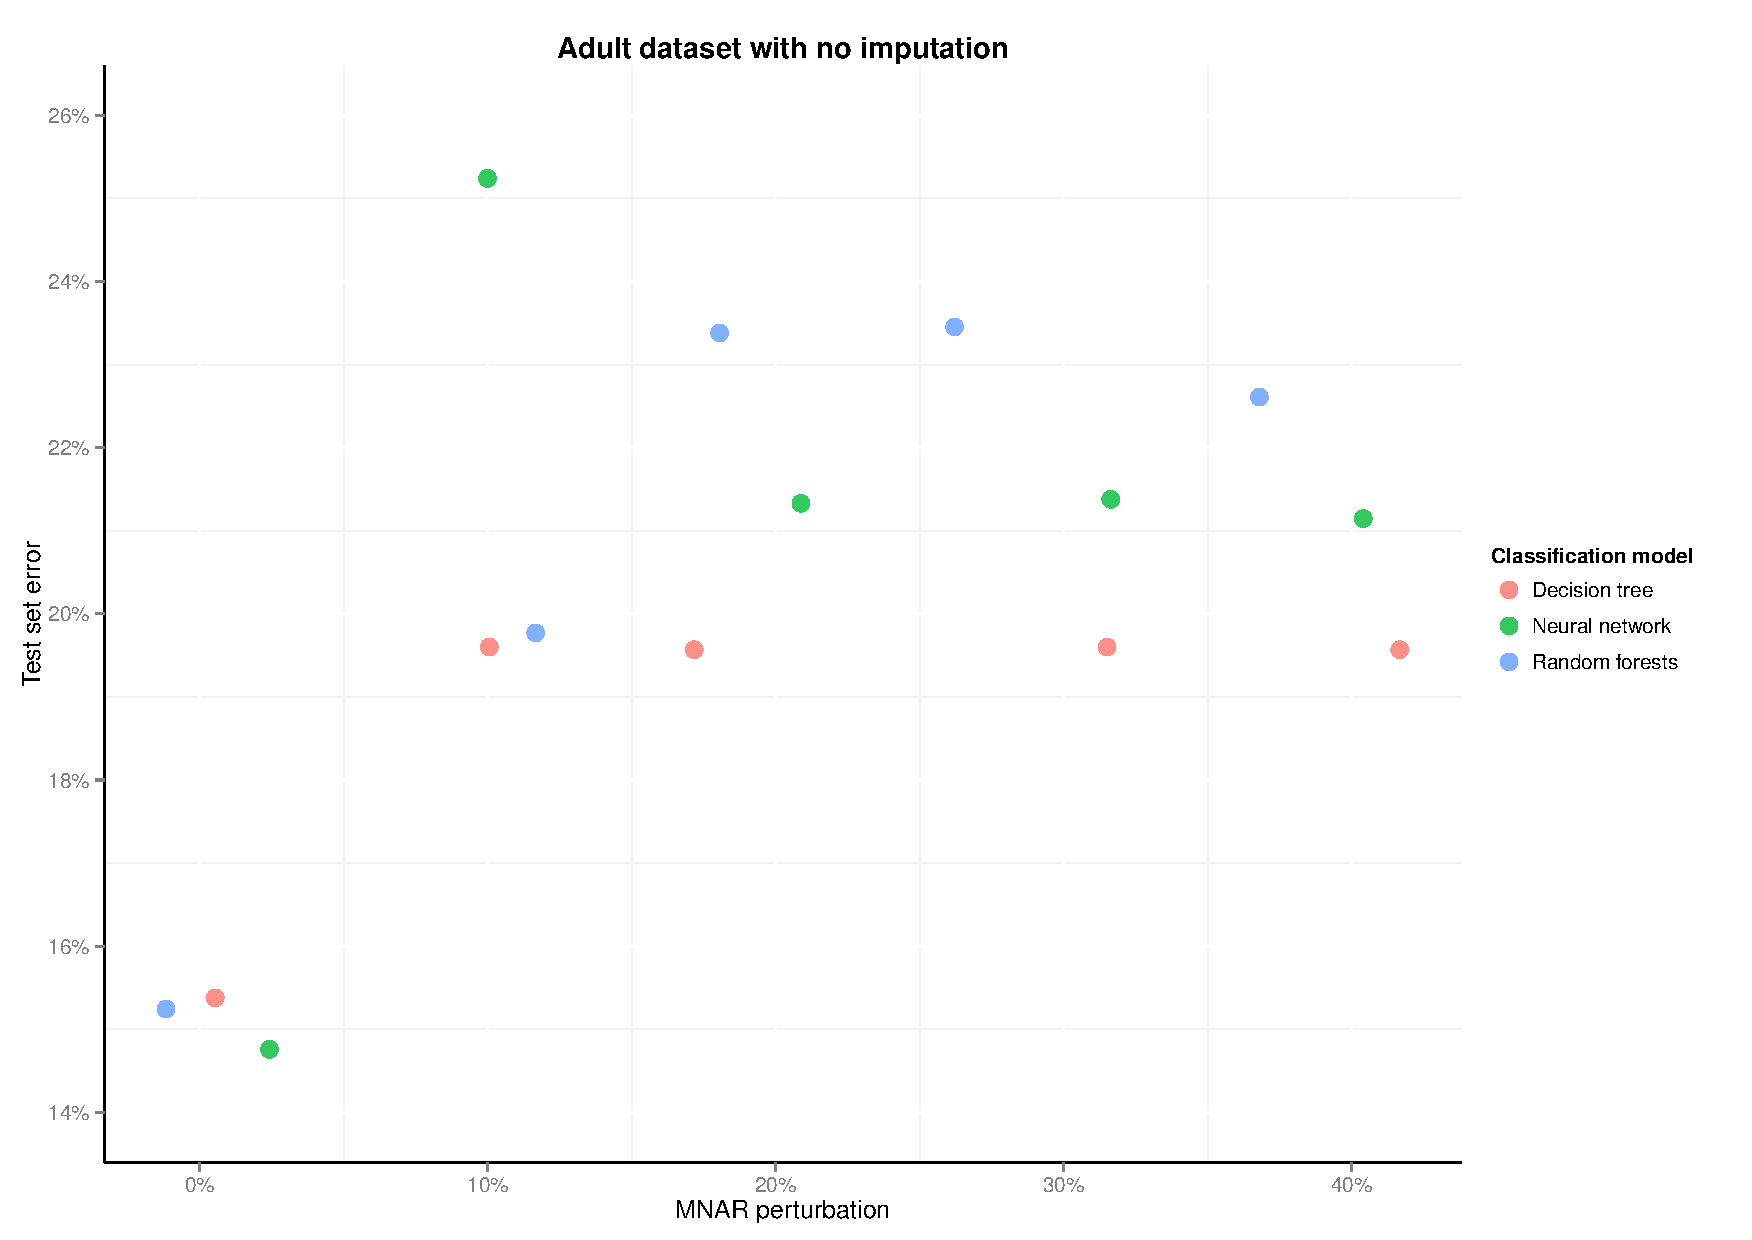
\includegraphics [scale=0.45]{figure/test-errors-adult-no-imp.pdf}\par
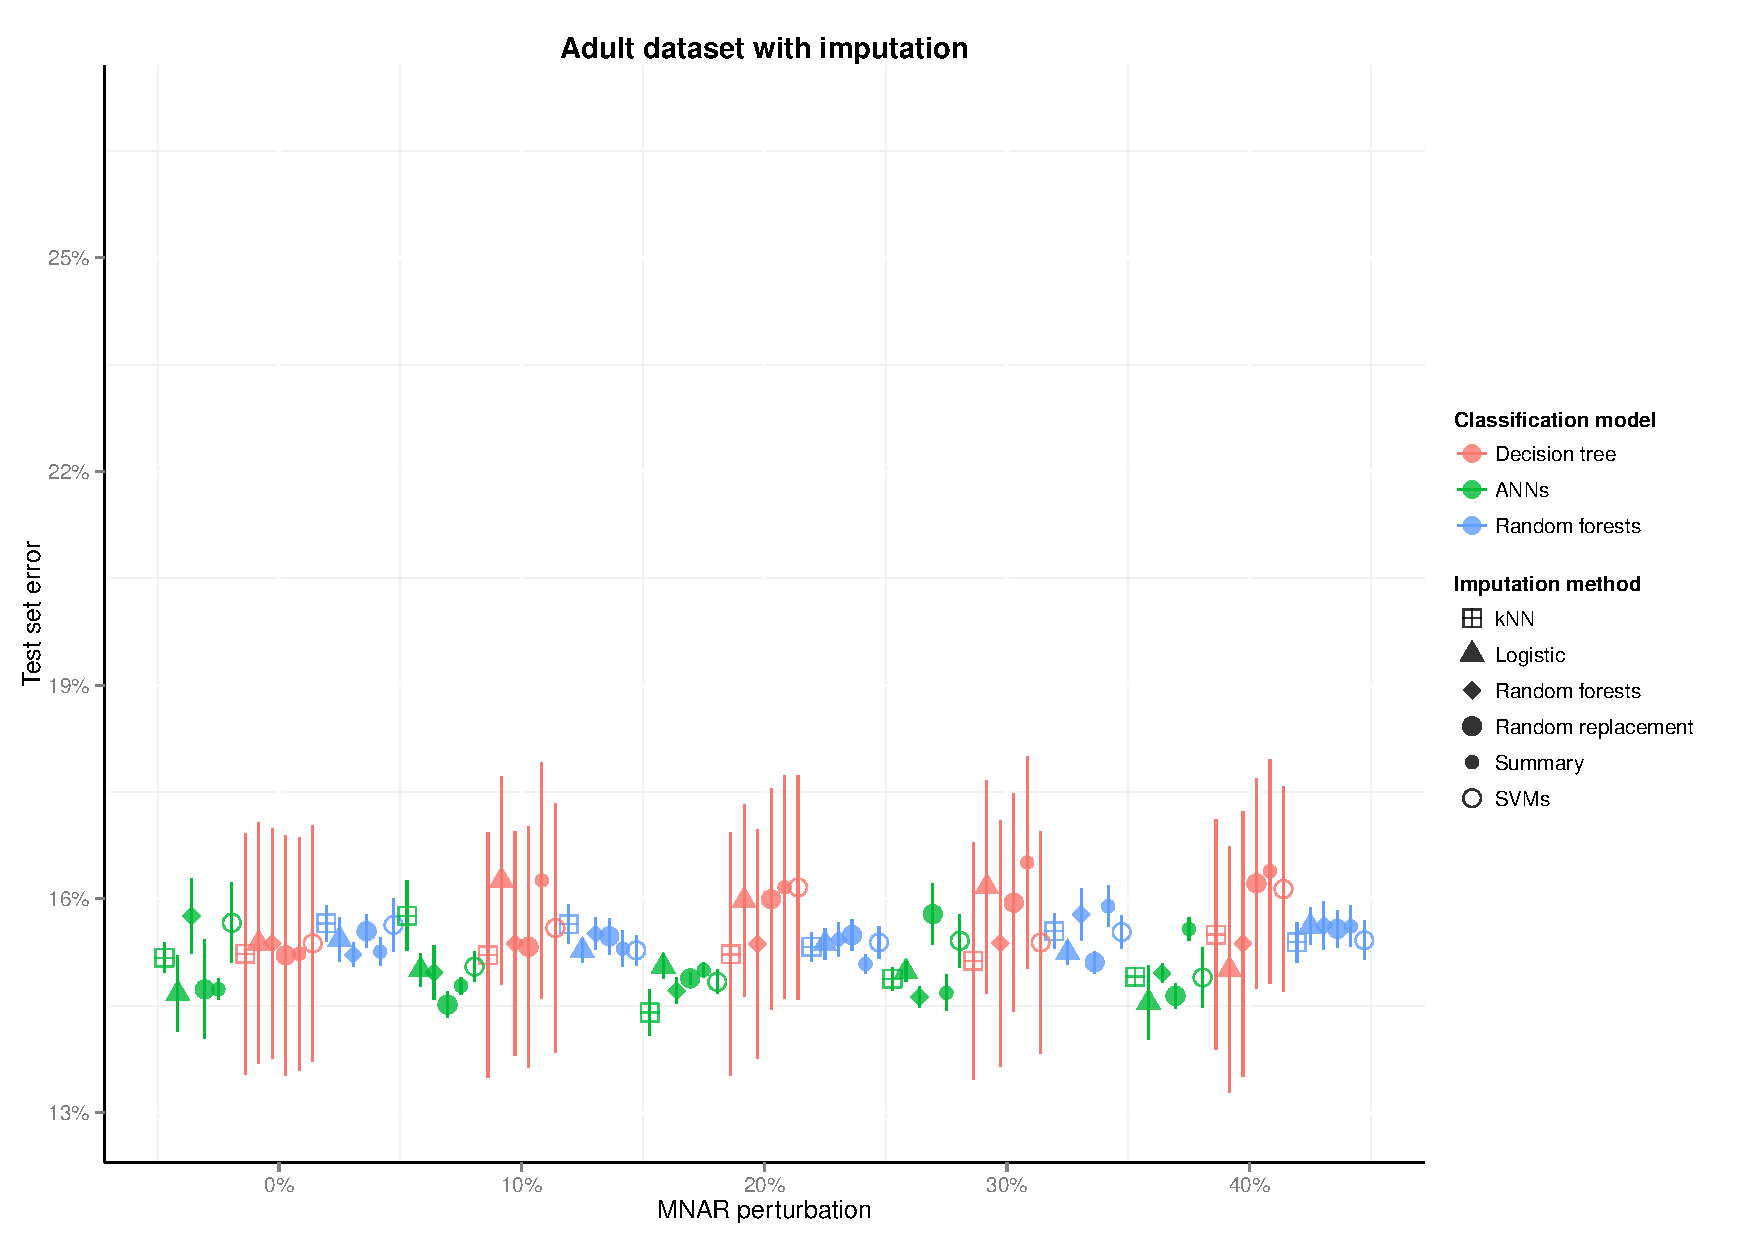
\includegraphics [scale=0.45]{figure/test-errors-adult-imp.pdf}\par
   \caption{\footnotesize Error rates on the Adult test set with (bottom) and without (top) missing data imputation, for various levels of MNAR-perturbed categorical training features (x-axis). One-hot encoding is used to represent missing data in the absence of imputation. Error bars represent one standard deviation from the test error prediction.}
   \label{fig:test-error-adult}
\end{figure}

\begin{figure}[h!]
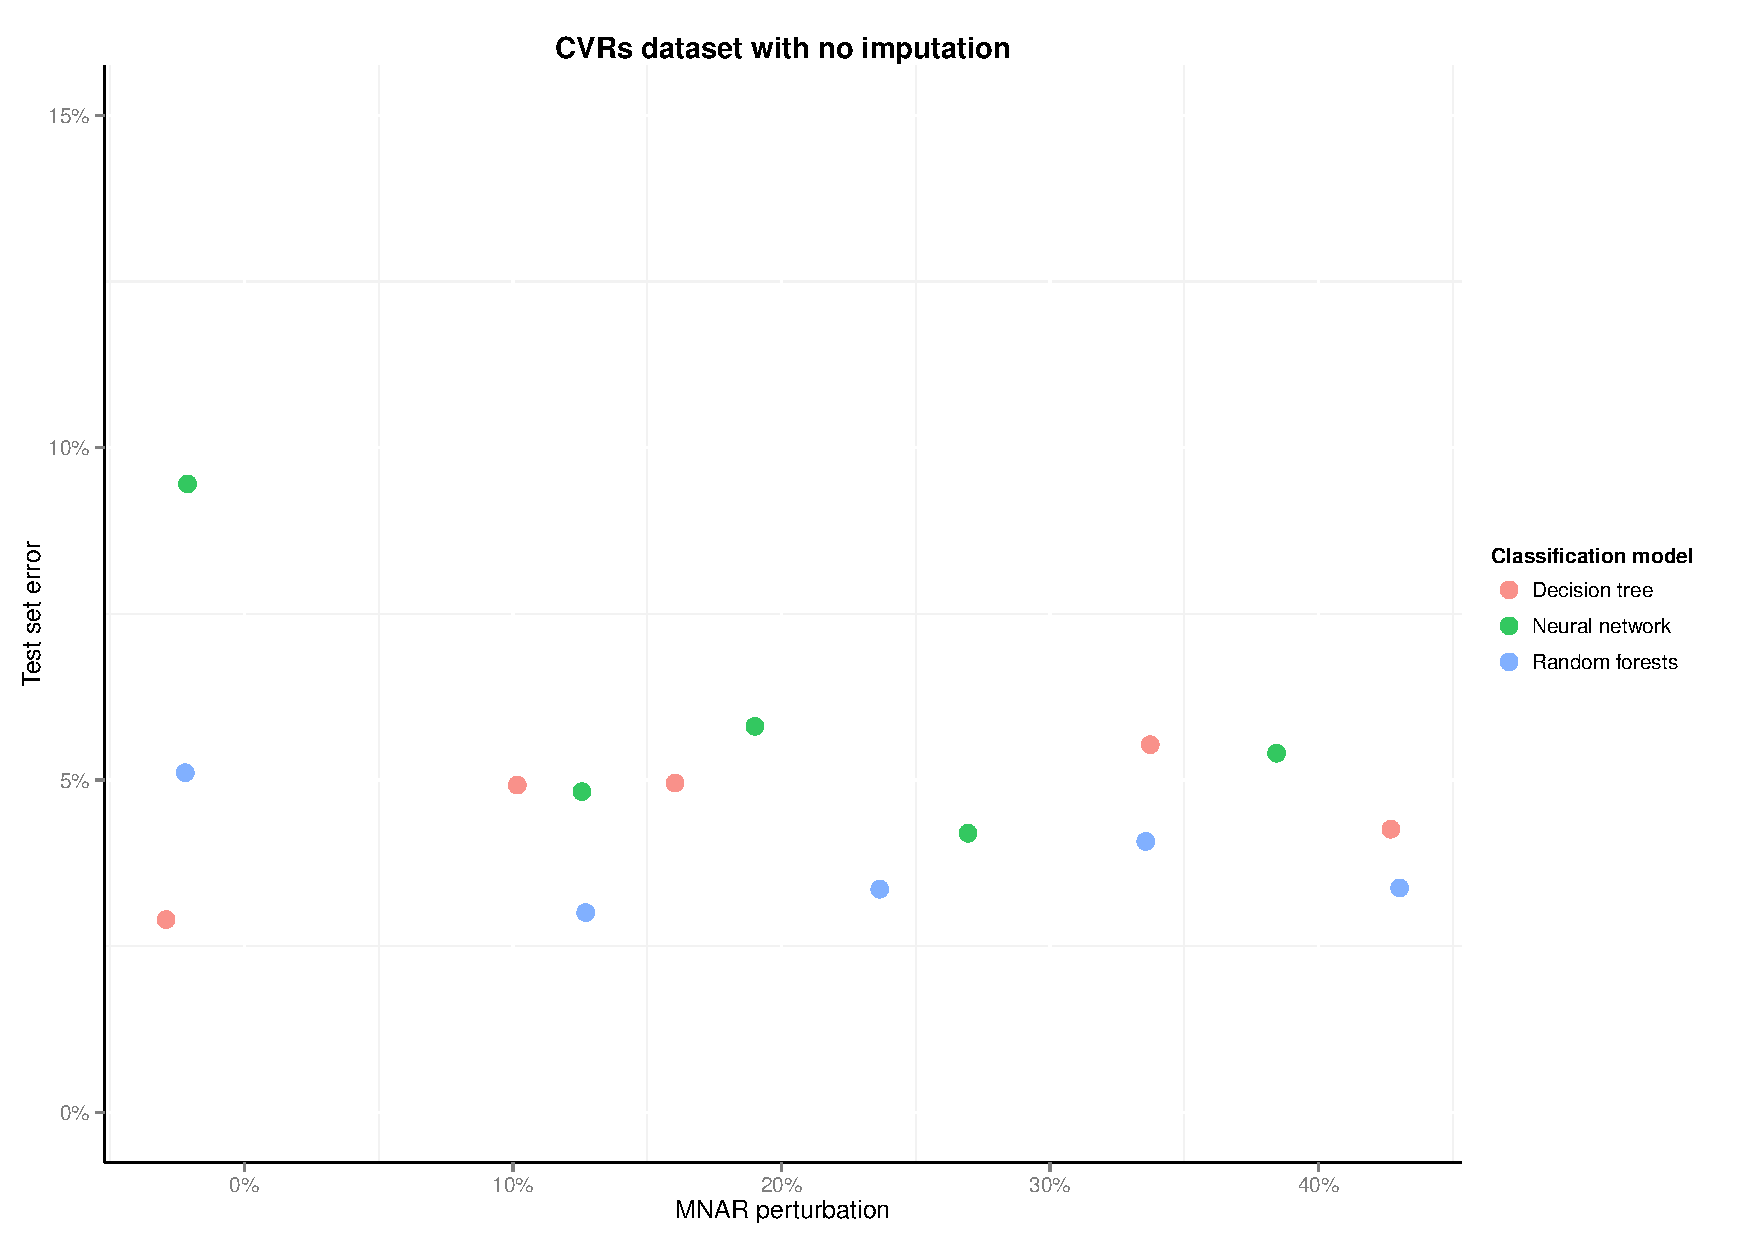
\includegraphics [scale=0.45]{figure/test-errors-votes-no-imp.pdf}\par
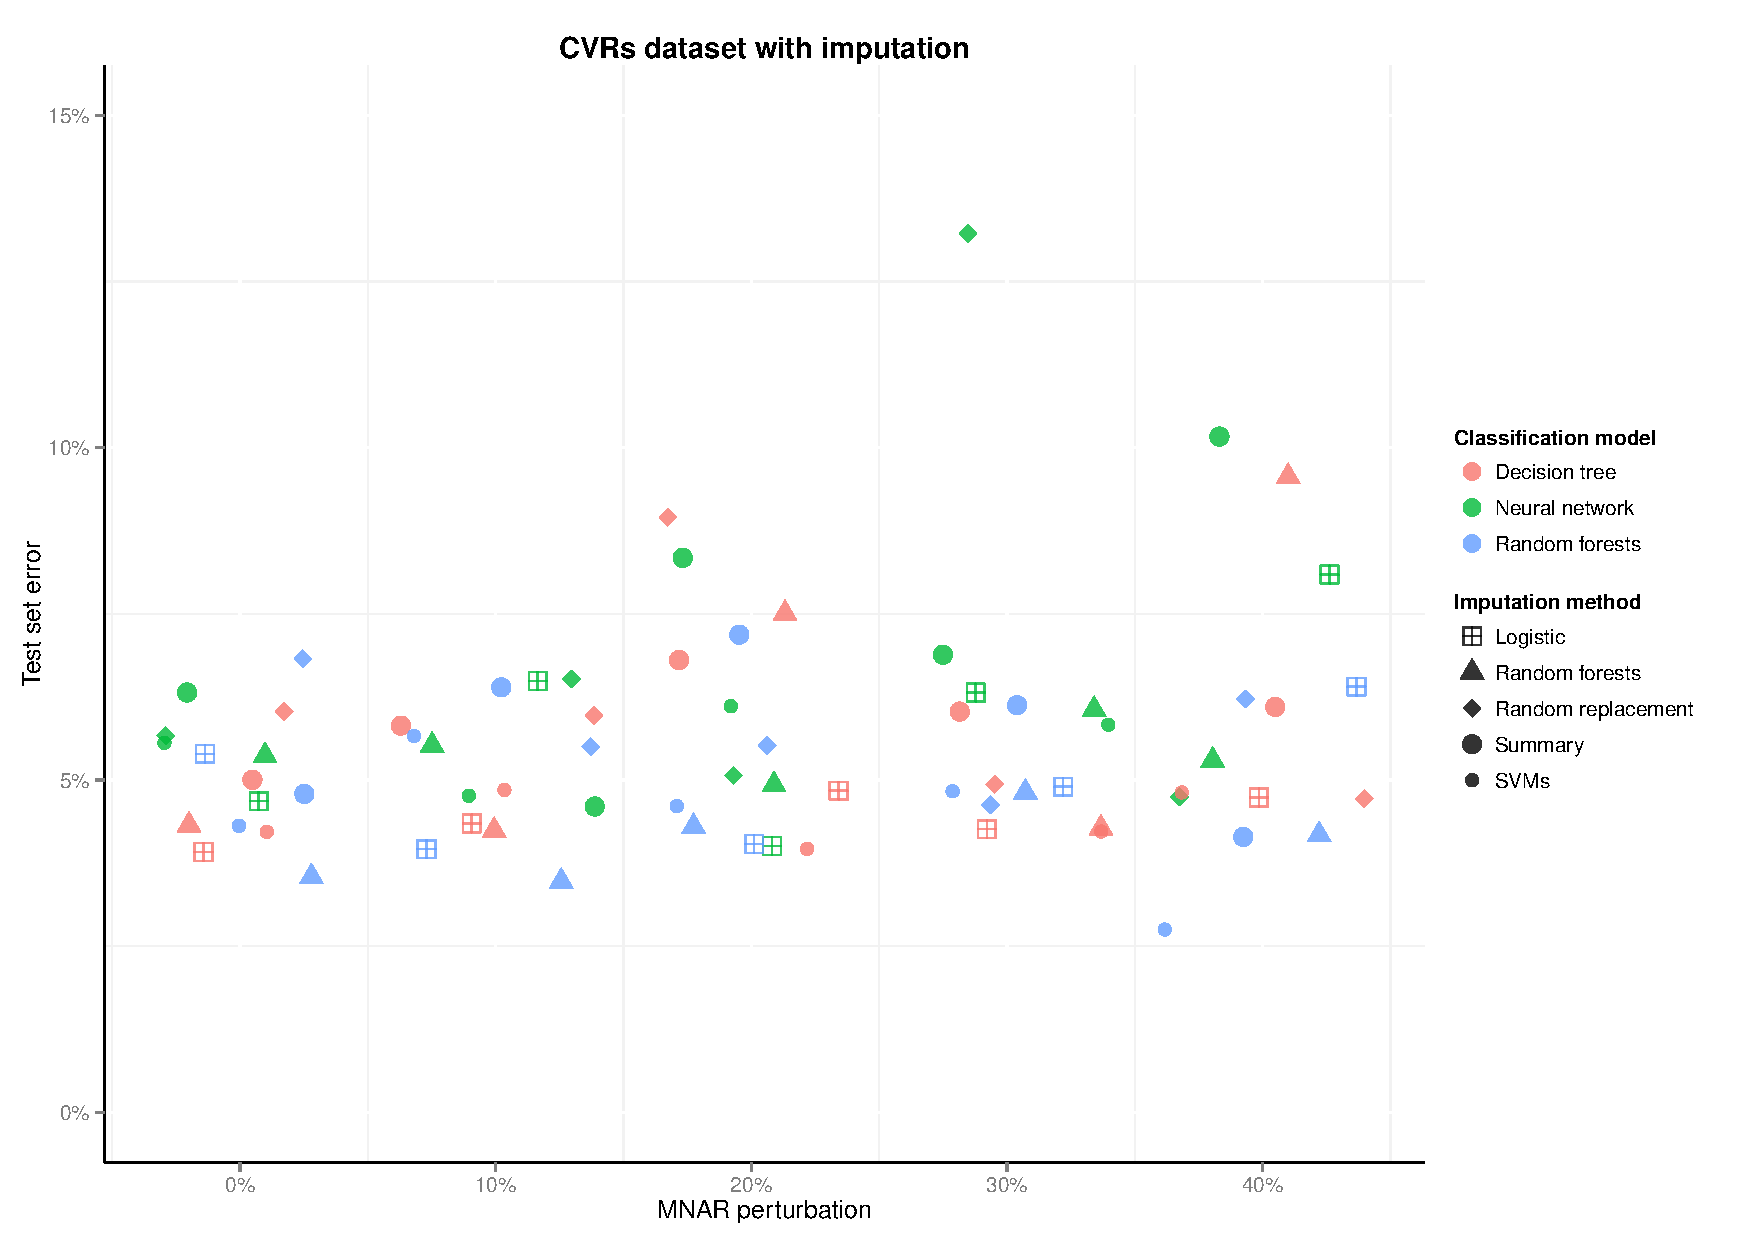
\includegraphics [scale=0.45]{figure/test-errors-votes-imp.pdf}\par
   \caption{\footnotesize Error rates on the CVRs test set with (bottom) and without (top) missing data imputation. See footnotes for Figure \ref{fig:test-error-adult}.}
   \label{fig:test-error-votes}
\end{figure}

\par

\setcounter{chapter}{4}
\setcounter{equation}{0} %-1
\noindent {\bf 4. Conclusion}  

This paper investigates the effects of missing data imputation and perturbation on classification tasks using supervised learning algorithms. We compare the predictive performance of ANNs against decision tree and random forest classifiers trained on datasets with differently imputed data. We assess performance in terms of test set error for different levels of MNAR-perturbed training data. We come close to beating the state-of-the-art test error on the Adult dataset using a ANN classifier trained on data imputed with $k$-NN  and outperform the state-of-the-art on the CVRs dataset by over 2\% using one-hot-encoded random forests. 

We conclude from the results that the performance of the classifiers and imputation strategies generally depend on the nature and proportion of missing data. For the Adult dataset, ANNs trained on imputed data outperform other classifiers and imputation methods across different ratios of perturbed data, while classifiers trained on one-hot encoded data perform very poorly on perturbed training data. This finding can be explained by the fact that one-hot encoding can bias estimates when the features are correlated, which is the case in the Adult dataset, but not CVRs dataset. 

Future work could help identify the conditions under which missing-data perturbation might improve prediction accuracy by acting as a regularization technique. The results of the present study show that perturbation can help increase predictive accuracy for imputed models, but not non-imputed models. Future work might compare missing-data perturbation with dropout training, which changes to zero all the values of a random subset of features \citep{hinton2012, maaten2013, wang2013}. 

\par
%%%%%%%%%%%%%%%%%%%%%%%%%%%%%%%%%%%%%%%%%%%%%%%%%%%%%%%%%%%%%%%%%%%%%%%%%%%%%%%%%%%%%%%%%%%%%%%%%%%%%%%%%%%%%%%%%%%%%%%%%%%%
\vskip 14pt
\noindent {\large\bf Supplementary Materials}

%Contain the brief description of the online supplementary materials.
The online supplementary material contains descriptive plots of missing data patterns in the benchmark datasets, and plots of Bayesian hyperparameter optimization for training ANNs on the benchmark datasets. The code used for this project is available on Github (\url{https://github.com/rafaelvalle/MDI}).

\par
%%%%%%%%%%%%%%%%%%%%%%%%%%%%%%%%%%%%%%%%%%%%%%%%%%%%%%%%%%%%%%%%%%%%%%%%%%%%%%%%%%%%%%%%%%%%%%%%%%%%%%%%%%%%%%%%%%%%%%%%%%%%
\vskip 14pt
\noindent {\large\bf Acknowledgements}

%Write the acknowledgements here.
We thank Isabelle Guyon for advice and the idea for the paper. We also thank Joan Bruna and seminar participants at the University of California, Berkeley, for comments. This material is based upon work supported by the National Science Foundation Graduate Research Fellowship under Grant No. DGE 1106400. Any opinion, findings, and conclusions or recommendations expressed in this material are those of the authors and do not necessarily reflect the views of the National Science Foundation.
\par

%%%%%%%%%%%%%%%%%%%%%%%%%%%%%%%%%%%%%%%%%%%%%%%%%%%%%%%%%%%%%%%%%%%%%%%%%%%%%%%%%%%%%%%%%%%%%%%%%%%%%%%%%%%%%%%%%%%%%%%%%%%%
\markboth{\hfill{\footnotesize\rm JASON POULOS AND RAFAEL VALLE} \hfill}
{\hfill {\footnotesize\rm MISSING DATA IMPUTATION} \hfill}

\bibhang=1.7pc
\bibsep=2pt
\fontsize{9}{14pt plus.8pt minus .6pt}\selectfont
\renewcommand\bibname{\large \bf References} 
\clearpage
\markboth{\hfill{\footnotesize\rm JASON POULOS AND RAFAEL VALLE} \hfill}
{\hfill {\footnotesize\rm MISSING DATA IMPUTATION} \hfill}
\begin{thebibliography}{11}
\expandafter\ifx\csname
natexlab\endcsname\relax\def\natexlab#1{#1}\fi
\expandafter\ifx\csname url\endcsname\relax
  \def\url#1{\texttt{#1}}\fi
\expandafter\ifx\csname urlprefix\endcsname\relax\def\urlprefix{URL
}\fi
\bibitem[Batista and Monard, 2003]{batista2003analysis}
Batista, G.~E. and Monard, M.~C. (2003).
\newblock An analysis of four missing data treatment methods for supervised
  learning.
\newblock {\em Applied Artificial Intelligence}, 17(5-6):519--533.

\bibitem[De~Leeuw et~al., 2003]{de2003prevention}
De~Leeuw, E.~D., Hox, J., Huisman, M., et~al. (2003).
\newblock Prevention and treatment of item nonresponse.
\newblock {\em Journal of Official Statistics}, 19(2):153--176.

\bibitem[Heskes et~al., 1997]{heskes1997}
Heskes, T., Wiegerinck, W., and Kappen, H. (1997).
\newblock Practical confidence and prediction intervals for prediction tasks.
\newblock In {\em Advances in Neural Information Processing Systems 9:
  Proceedingss of the 1996 Conference}. MIT Press.

\bibitem[Hinton et~al., 2012]{hinton2012}
Hinton, G.~E., Srivastava, N., Krizhevsky, A., Sutskever, I., and
  Salakhutdinov, R.~R. (2012).
\newblock Improving neural networks by preventing co-adaptation of feature
  detectors.
\newblock {\em arXiv preprint arXiv:1207.0580}.

\bibitem[Jones, 1996]{jones1996}
Jones, M.~P. (1996).
\newblock Indicator and stratification methods for missing explanatory
  variables in multiple linear regression.
\newblock {\em Journal of the American Statistical Association},
  91(433):222--230.

\bibitem[Kohavi, 1996]{kohavi1996}
Kohavi, R. (1996).
\newblock Scaling up the accuracy of naive-bayes classifiers: A decision-tree
  hybrid.
\newblock In {\em Proceedings of the Second International Conference on
  Knowledge Discovery and Data Mining}, pages 202--207. Citeseer.

\bibitem[Li et~al., 2004]{li2004}
Li, D., Deogun, J., Spaulding, W., and Shuart, B. (2004).
\newblock Towards missing data imputation: a study of fuzzy k-means clustering
  method.
\newblock In {\em International Conference on Rough Sets and Current Trends in
  Computing}, pages 573--579. Springer.

\markboth{\hfill{\footnotesize\rm JASON POULOS AND RAFAEL VALLE} \hfill}
{\hfill {\footnotesize\rm MISSING DATA IMPUTATION} \hfill}
\bibitem[Lichman, 2013]{Lichman2013}
Lichman, M. (2013).
\newblock {UCI} {M}achine {L}earning {R}epository.

\bibitem[Little and Rubin, 2014]{little2014}
Little, R.~J. and Rubin, D.~B. (2014).
\newblock {\em Statistical Analysis with Missing Data}.
\newblock John Wiley \& Sons.

\bibitem[Maaten et~al., 2013]{maaten2013}
Maaten, L., Chen, M., Tyree, S., and Weinberger, K.~Q. (2013).
\newblock Learning with marginalized corrupted features.
\newblock In {\em Proceedings of the 30th International Conference on Machine
  Learning (ICML-13)}, pages 410--418.

\bibitem[Rubin et~al., 1995]{rubin1995}
Rubin, D.~B., Stern, H.~S., and Vehovar, V. (1995).
\newblock Handling \enquote{don't know} survey responses: the case of the
  {S}lovenian plebiscite.
\newblock {\em Journal of the American Statistical Association},
  90(431):822--828.

\bibitem[Schlimmer, 1987]{schlimmer1987}
Schlimmer, J.~C. (1987).
\newblock {\em Concept Acquisition Through Representational Adjustment}.
\newblock PhD thesis, Department of Information and Computer Science,
  University of California, Irvine.

\bibitem[Schlimmer and Granger~Jr, 1986]{schlimmer1986}
Schlimmer, J.~C. and Granger~Jr, R.~H. (1986).
\newblock Incremental learning from noisy data.
\newblock {\em Machine learning}, 1(3):317--354.

\bibitem[Silva-Ram{\'\i}rez et~al., 2011]{silva2011}
Silva-Ram{\'\i}rez, E.-L., Pino-Mej{\'\i}as, R., L{\'o}pez-Coello, M., and
  Cubiles-de-la Vega, M.-D. (2011).
\newblock Missing value imputation on missing completely at random data using
  multilayer perceptrons.
\newblock {\em Neural Networks}, 24(1):121--129.

\bibitem[Snoek et~al., 2012]{snoek2012}
Snoek, J., Larochelle, H., and Adams, R.~P. (2012).
\newblock Practical {B}ayesian optimization of machine learning algorithms.
\newblock In {\em Advances in neural information processing systems}, pages
  2951--2959.

\bibitem[Tsiatis, 2007]{tsiatis2007}
Tsiatis, A. (2007).
\newblock {\em Semiparametric Theory and Missing Data}.
\newblock Springer Science \& Business Media.

\bibitem[Wang and Manning, 2013]{wang2013}
Wang, S. and Manning, C. (2013).
\newblock Fast dropout training.
\newblock In {\em Proceedings of the 30th International Conference on Machine
  Learning (ICML-13)}, pages 118--126.

\bibitem[Zeiler, 2012]{zeiler2012}
Zeiler, M.~D. (2012).
\newblock Adadelta: an adaptive learning rate method.
\newblock {\em arXiv preprint arXiv:1212.5701}.

%%%%%%%%%%%%%%%%%%%%%%%%%%%%%%%%%%%%%%%%%%%%%%%%%%%%%%%%%%%%%%%%%%%%%%%%%%%%%%%%%%%%%%%%%%%%%%%%%%%%%%%%%%%%%%%%%%%%%%%%%%%%
\end{thebibliography}

%\bibliographystyle{apalike}
%\bibliography{refs}

\vskip .65cm
\noindent
Department of Political Science, University of California, Berkeley, CA 94720-1950
\vskip 2pt
\noindent
E-mail: \href{mailto:poulos@berkeley.edu}{\nolinkurl{poulos@berkeley.edu}}
\vskip 2pt

\noindent
Center for New Music and Audio Technologies, University of California, Berkeley, CA 94720
\vskip 2pt
\noindent
E-mail: \href{mailto:rafaelvalle@berkeley.com}{\nolinkurl{rafaelvalle@berkeley.com}}
% \vskip .3cm
%\centerline{(Received ???? 20??; accepted ???? 20??)}\par
\end{document}
%%%%%%%%%%%%%%%%%%%%%%%%%%%%%%%%%%%%%%%%%%%%%%%%%%%%%%%%%%%%%%%%%%%%%%%%%%%%%%%%%%%%%%%%%%%%%%%%%%%%%%%%%%%%%%%%%%%%%%%%%%%%
%%%%%%%%%%%%%%%%%%%%%%%%%%%%%%%%%%%%%%%%%%%%%%%%%%%%%%%%%%%%%%%%%%%%%%%%%%%%%%%%%%%%%%%%%%%%%%%%%%%%%%%%%%%%%%%%%%%%%%%%%%%%

\end{document}
